\section{Conventions used in this document}
\label{sec:conventions}

% ~~~~~~~~~~~~~~~~~~~~~~~~~~~~~~~~~~~~
% UML
% ~~~~~~~~~~~~~~~~~~~~~~~~~~~~~~~~~~~~
\subsection{UML classes}
A SED-ML UML class (\fig{umlClass}) consists of a class name (\code{ClassName}) and a number of attributes (\code{attribute}) each of a specific data type (\code{type}). The SED-ML UML specification does not make use of UML \code{operations}. SED-ML class names always begin with upper case letters. If they are composed of different words, the camel case style is used, as in e.\,g.\ \code{DataGenerator}.
\begin{figure}[ht]
	\centering
	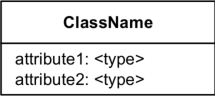
\includegraphics[width=0.25\textwidth]{images/uml/umlClass}
	\caption{UML class}
	\label{fig:umlClass}    
\end{figure}

% ~~~~~~~~~~~~~~~~~~~~~~~~~~~~~~~~~~~~
% UML RELATIONSHIPS
% ~~~~~~~~~~~~~~~~~~~~~~~~~~~~~~~~~~~~
\subsection{UML relationships}
\subsubsection{UML relation types}
Links between classes specify the connection of objects with each other (\fig{umlRelationships}). The different relation types used in the SED-ML specification include aggregation, composite aggregation, and generalisation. The label on the line is called symbol (\code{label}) and describes the relation of the objects of both classes. 

\begin{figure}[ht]
	\centering
	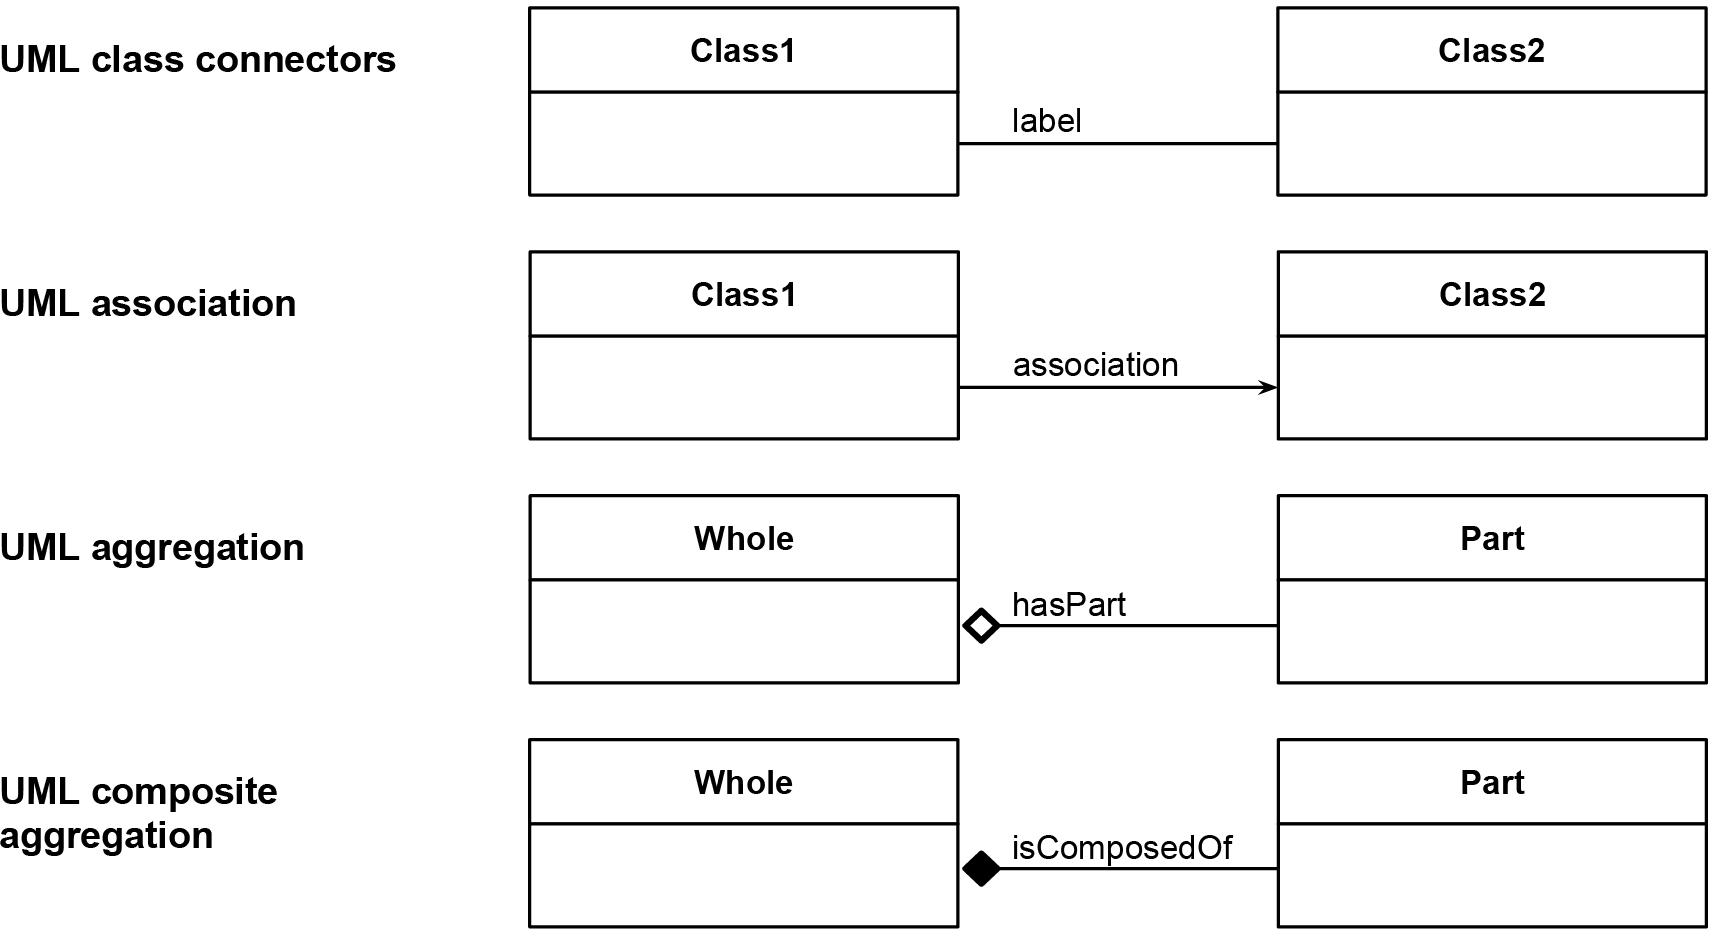
\includegraphics[width=0.8\textwidth]{images/uml/umlRelationship}
	\caption{UML class connectors, association, aggregation, composite aggregation}
	\label{fig:umlRelationships}
\end{figure}

% ~~~ ASSOCIATION ~~
The \concept{association} (\fig{umlRelationships}) indicates the existence of a connection between the objects of the participating classes. Often associations are directed to show how the label should be read (in which direction). Associations can be uni-directional (one arrowhead), or bidirectional (zero or two arrowheads).
  
% ~~~ AGGREGATION ~~~
The \concept{aggregation} (\fig{umlRelationships}, top) indicates that the objects of the participating classes are connected in a way that one class (\code{Whole}) consists of several parts (\code{Part}).

% ~~~ COMPOSITE AGGREGATION ~~~
The \concept{composite aggregation} (\fig{umlRelationships}, bottom) indicates that the objects of the participating classes are connected in a way that one class (\code{Whole}) consists of several parts (\code{Part}). In contrast to the aggregation, the subelements (\code{Part}) are dependent on the parent class (\code{Whole}).

% ~~~ INHERITANCE ~~~
The \concept{generalisation} (\fig{umlGeneralisation}) allows to extend classes (\code{BaseClass}) by additional properties. The derived class (\code{DerivedClass}) inherits all properties of the base class.

\begin{figure}[h]
	\centering
	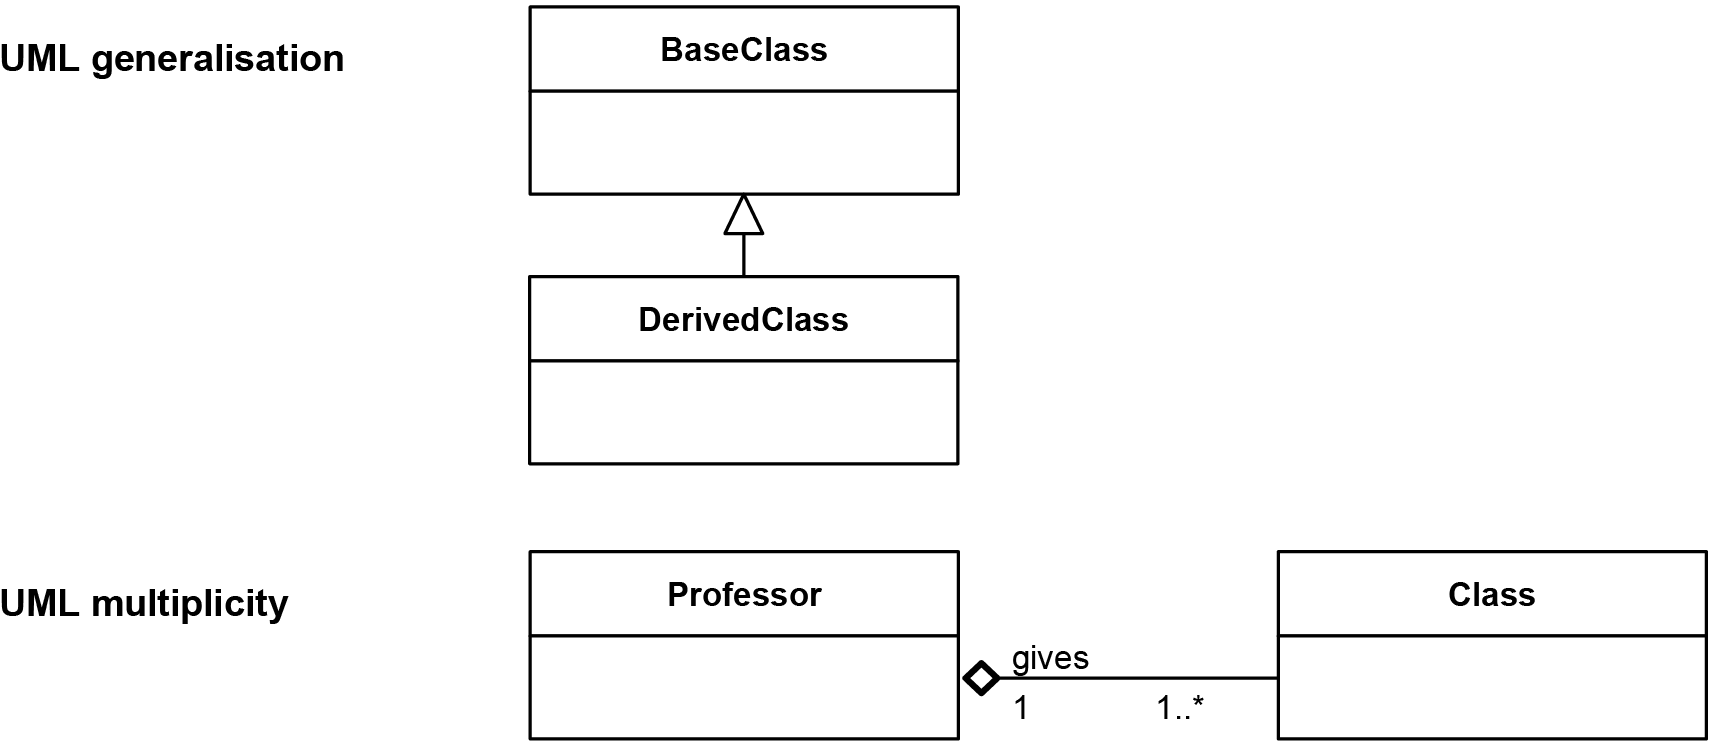
\includegraphics[width=0.8\textwidth]{images/uml/umlGeneralisation}
	\caption{UML generalisation (top) and multiplicity (bottom)}
	\label{fig:umlGeneralisation}
\end{figure}


%% ~~~ UML MULTIPLICITY ~~~
\subsubsection{UML multiplicity}
UML multiplicity (\fig{umlGeneralisation} defines the number of objects in one class that can be related to one object in the other class (also known as \concept{cardinality}). Possible types of multiplicity include values (1), ranges (1$..$4), intervals (1,3,9), or combinations of ranges and intervals. The standard notation for ``many'' is the asterisk (*). 

Multiplicity can be defined for both sides of a relationship between classes. The default relationship is ``many to many''. The example in \fig{umlGeneralisation} (bottom) expresses that a class is given by a professor, and a professor might give one to many classes.


% ~~~~~~~~~~~~~~~~~~~~~~~~~~~~~~~~~~~~
% XML SCHEMA
% ~~~~~~~~~~~~~~~~~~~~~~~~~~~~~~~~~~~~
\subsection{XML schema language elements}
The main building blocks of an XML Schema specification are simple and complex types, element specifications and attribute specifications.

XML Schema \concept{definitions} create new types, \concept{declarations} define new elements and attributes.
The definition of new (simple and complex) types can be based on a number of already existing, predefined types (string, boolean, float). Simple types are restrictions or extensions of predefined types. Complex types describe how attribues can be assigned to elements and how elements can contain further elements. The current SED-ML XML Schema only makes use of \emph{complex type definitions}. An example for a complex type definition is given in \lst{complexType}:

\begin{myXmlLst}{Complex Type definition of the SED-ML \code{computeChange} element}{lst:complexType}
<xs:element name="computeChange">
	<xs:complexType>
		<xs:complexContent>
			<xs:extension base="SEDBase">
				<xs:sequence>
					<xs:element ref="listOfVariables" minOccurs="0" />
					<xs:element ref="listOfParameters" minOccurs="0" />
					<xs:element ref="math" />
				</xs:sequence>
				<xs:attribute name="target" use="required" type="xs:token" />
			</xs:extension>
		</xs:complexContent>
	</xs:complexType>
</xs:element>
\end{myXmlLst}

It shows the declaration of the element \code{computeChange} that is used in SED-ML to change mathematical expressions. The element is defined using an \emph{unnamed} complex type which is built of further elements called \code{listOfVariables}, \code{listOfParameters}, and \code{math}. Additionally, the element \code{computeChange} has an attribute \code{target}. The definition of the elements inside the complex type are defined elsewhere in the schema and only referred to in the definition of \code{ComputeChange}.

The nesting of elements in the schema can be expressed using the concepts \code{xs:sequence} (a sequence of elements), \code{xs:choice} (an alternative of elements to choose from), or \code{xs:all} (a set of elements that can occur in any order). The current SED-ML XML Schema only uses the \emph{sequence} of elements. 


%% ~~~ MULTIPLICITIES ~~~
\subsubsection{Multiplicities}
The standard multiplicity for each defined \code{element} is 1. Explicit multiplicity is defined using the \code{minOccurs} and \code{maxOccurs} attributes inside the complex type definition, as shown in \lst{multiplicity}.

\begin{myXmlLst}{Multiplicity for complex types in XML Schema}{lst:multiplicity}
<xs:element name="dataGenerator">
	<xs:complexType>
		<xs:complexContent>
			<xs:extension base="SEDBase">
				<xs:sequence>
					<xs:element ref="listOfVariables" minOccurs="0" />
					<xs:element ref="listOfParameters" minOccurs="0" />
					<xs:element ref="math" />
				</xs:sequence>
				<xs:attributeGroup ref="idGroup" />
			</xs:extension>
		</xs:complexContent>
	</xs:complexType>
</xs:element>
\end{myXmlLst}

In this example, the \code{dataGenerator} type is build of a sequence of three elements: The \code{listOfVariables} element is not necessary for the definition of a valid \code{dataGenerator} XML structure (it may occur 0 times or once). The same is true for the \code{listOfParameters} element (it may as well occur 0 times or once). The \code{math} element, however, uses the implicit standard multiplicity -- it must occur exactly 1 time in the \code{dataGenerator} specification.

%% ~~~ TYPE EXTENSIONS ~~~
\subsection{Type extensions}
XML Schema offers mechanisms to restrict and extend previously defined complex types. Extensions add element or attribute declarations to existing types, while restrictions restrict the types by adding further characteristics and requirements (facets) to a type. An example for a type extension is given in \lst{xmlExtension}.

\begin{myXmlLst}{Definition of the sedML type through extension of SEDBase in SED-ML}{lst:xmlExtension}
<xs:element name="sedML">
	<xs:complexType>
		<xs:complexContent>
			<xs:extension base="SEDBase">
				<xs:sequence>
					<xs:element ref="listOfSimulations" minOccurs="0" />
					<xs:element ref="listOfModels" minOccurs="0" />
					<xs:element ref="listOfTasks" minOccurs="0" />
					<xs:element ref="listOfDataGenerators" minOccurs="0" />
					<xs:element ref="listOfOutputs" minOccurs="0" />
				</xs:sequence>
				<xs:attribute name="level" type="xs:decimal" use="required"
					fixed="1" />
				<xs:attribute name="version" type="xs:decimal" use="required"
					fixed="2" />
			</xs:extension>
		</xs:complexContent>
	</xs:complexType>
</xs:element>
\end{myXmlLst}

The \code{sedML} element is an extension of the previously defined \code{SEDBase} type. It extends \code{SEDBase} by a sequence of five additional elements (\code{listOfSimulations}, \code{listOfModels}, \code{listOfTasks}, \code{listOfDataGenerators}, and \code{listOfOutputs}) and two new attributes \code{version} and \code{level}.
